\documentclass[twoside,10pt]{article}
\usepackage{/Users/bradenhoagland/latex/styles/toggles}
%\toggletrue{sectionbreaks}
%\toggletrue{sectionheaders}
\newcommand{\docTitle}{HW 3}
\usepackage{/Users/bradenhoagland/latex/styles/common}
\importStyles{modern}{rainbow}{boxy}

%\renewcommand{\theenumi}{\alph{enumi}}

\begin{document}
%\tableofcontents

% ------------------------------
% 1.58
% ------------------------------
\begin{exer}[1.58]
Area of arbelos.
\end{exer}

By symmetry, doubling $CD$ gives a chord of the circle. Then by power of the point,
\[
|AC| |CB| = |CD|^2.
\] Then the area of the arbelos is
\begin{align*}
	\text{Area}(\text{arbelos}) &= \frac{\pi}{2} \left[ \left( \frac{|AC|+|CB|}{2}  \right)^2 - \left(\frac{|AC|}{2}\right)^2 - \left( \frac{|CB|}{2}  \right)^2\right] \\
				    &= \frac{\pi}{4} |AC| |CB| \\
				    &= \frac{\pi}{4} |CD|^2 \\
				    &= \pi \left( \frac{|CD|}{2}  \right)^2 \\
				    &= \text{Area}(\text{circle with diameter } CD).
\end{align*}

\newpage

% ------------------------------
% 1.71
% ------------------------------
\begin{exer}[1.71]
Diagonals of parallelogram bisect each other.
\end{exer}

\begin{figure}[H]
	\centering
	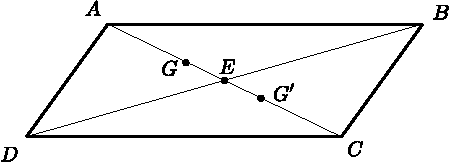
\includegraphics[scale=0.8]{fig/71.pdf}
	%\caption{}
\end{figure}

Let $E$ be the midpoint of $BD$, and let $G$ be the centroid of $\Delta ABD$. Then by Theorem 1.9.1, $|AE| = |AG| + |GE| = 3 |GE|$. By SSS, $\Delta ABD \cong \Delta CDB$. Thus if $G'$ is the centroid of $\Delta CDB$, we have $|G'E| = |GE|$. Then $|CE| = 3 |G'E| = 3 |GE| = |AE|$.

By a similar argument, $|BE|=|ED|$, so the diagonals bisect each other.

\newpage

% ------------------------------
% 1.79
% ------------------------------
\begin{exer}[1.79]
$I$ and $I_{a}$ both lie on $\Gamma$.
\end{exer}

\begin{figure}[H]
	\centering
	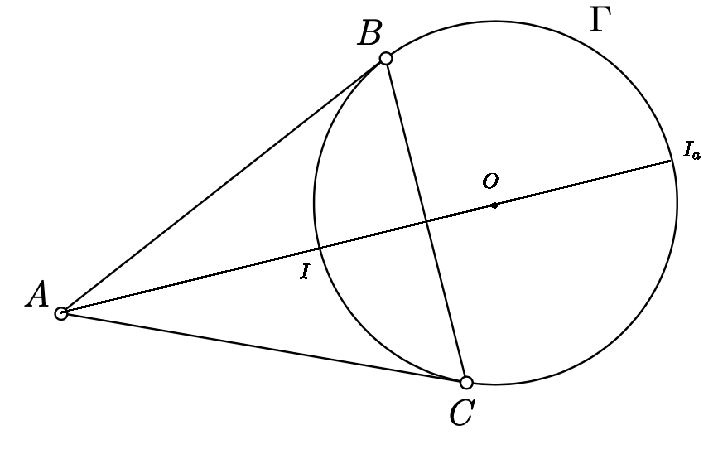
\includegraphics[scale=0.7]{fig/79.pdf}
	%\caption{}
\end{figure}

Let $O$ be the center of $\Gamma$. By symmetry, $AO$ bisects $\angle BAC$.

\textbf{Incenter:} Since $\angle CBA$ subtends the arc $BC$, $BC$'s measure is $2\angle CBA$. Then since $I$ is the midpoint of $BC$, $\angle IBA = \frac{1}{2} \angle CBA$. Thus $I$ is the intersection point of lines bisecting $\angle BAC$ and $\angle CBA$, so $I$ is the incenter.

\textbf{Excenter:} The exterior angle at $C$ subtends the large arc $BC$ (passing through $I_{a}$). By symmetry again, $I_{a}$ is the midpoint of that arc. Then $BI_{a}$ bisects the exterior angle at $B$. Since $I$ is a point of $A$'s angle bisector and $B,C$'s exterior angle bisectors, $I_{a}$ is an excenter.

\newpage

% ------------------------------
% 1.80
% ------------------------------
\begin{exer}[1.80]
	$|\Delta ABC| = (s-a)r_{a}$.
\end{exer}

\begin{figure}[H]
	\centering
	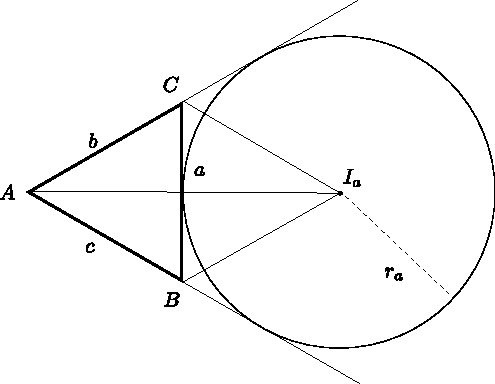
\includegraphics[scale=1]{fig/80.pdf}
	%\caption{}
\end{figure}

Consider the quadrilateral $ACI_{a}B$. Its area is
\[
|ACI_{a}B| = |\Delta ABC| + |\Delta BCI_{a}| = |\Delta ABI_{a}|+|\Delta ACI_{a}|,
\] so
\begin{align*}
	|\Delta ABC| &= |\Delta ABI_{a}| +|\Delta ACI_{a}| - |\Delta BCI_{a}| \\
		     &= \frac{1}{2} cr_{a} + \frac{1}{2} br_{a} - \frac{1}{2} ar_{a} \\
		     &= \frac{1}{2} (-a+b+c)r_{a} \\
		     &= (s-a)r_{a}.
\end{align*}

\newpage

% ------------------------------
% 1.81
% ------------------------------
\begin{exer}[1.81]
Distance from $A$ to a bunch of tangent things.
\end{exer}

In all three problems, the diagrams are set up so that we have to find $|AD|$.
\begin{enumerate}
	\item
		\begin{figure}[H]
			\centering
			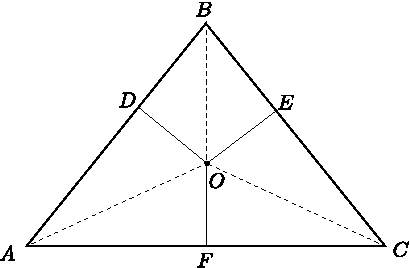
\includegraphics[scale=1]{fig/81a.pdf}
			%\caption{}
		\end{figure}
		By Theorem 1.10.3, $|\Delta ABC| = sr$. But after drawing altitudes from $O$, we get three pairs of congruent triangles. Thus we can also calculate $|\Delta ABC| = |AD|r+|BE|r+|CE|r = (|AD|+a)r$, so
		\[
			sr = (|AD|+a)r \implies |AD| = s-a.
		\] 

	\item 
		\begin{figure}[H]
			\centering
			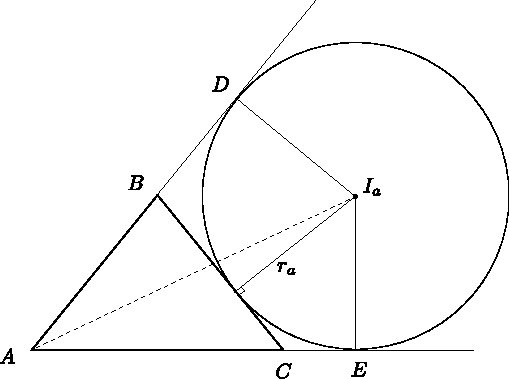
\includegraphics[scale=1]{fig/81b.pdf}
			%\caption{}
		\end{figure}
		By Exercise 1.80, $|\Delta ABC| = (s-a)r_{a}$. But the area of the quadrilateral $BDEC$ is $r_a a$, so $|\Delta ABC|=\frac{1}{2} |AD|r_{a} + \frac{1}{2} |AE|r_{a}-r_{a}a$. Since $|AD|=|AE|$ by symmetry, these two expressions for $|\Delta ABC|$ give
		\[
			(s-a)r_{a} = (|AD|-a)r_{a} \implies |AD|=s.
		\] 
	\item 
		\begin{figure}[H]
			\centering
			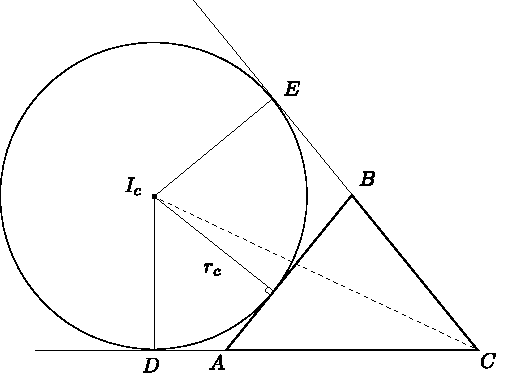
\includegraphics[scale=1]{fig/81c.pdf}
			%\caption{}
		\end{figure}
		A clear extension of Exercise 1.80 is $|\Delta ABC| = (s-c)r_{c}$. But we also have $|\Delta ABC| = (b+|AD|)r_{c} - cr_{c}$ via an argument similar to that in part (b). This gives
		\[
			(b+|AD|-c)r_{c} = (s-c)r_{c} \implies |AD| = s-b.
		\] 
\end{enumerate}

\newpage

% ------------------------------
% 1.100
% ------------------------------
\begin{exer}[1.100]
Putnam problem.
\end{exer}

\begin{figure}[H]
	\centering
	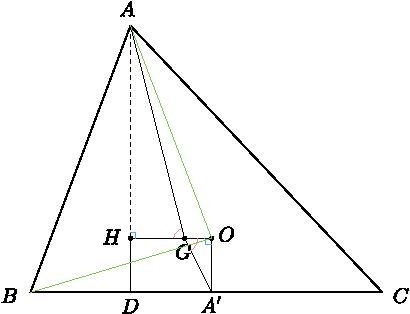
\includegraphics[scale=1]{fig/100.pdf}
	%\caption{}
\end{figure}

By the Euler Line theorem, the centroid $G$ lies on $HO$ and gives the ratio
\[
\frac{|OG|}{|GH|} = \frac{1}{2} .
\] Note that since the two pink angles and the two blue angles are equal, $\Delta AGH \sim \Delta A'GO$. Then we can use the above ratio, along with the given fact $|A'D|=5$, to get
\[
\frac{|A'O|}{|AH|} = \frac{|OG|}{|GH|} \implies |AH| = 10.
\] Then by the Pythagorean Theorem, $|AO|^2 = |AH|^2 + |HO|^2 = 221$. Since $O$ is the circumcenter, $|AO|=|BO|$. Then by the Pythaogrean Theorem again,
\begin{align*}
	|BA'|^2 + |A'O|^2 &= |BO|^2 \\
	|BA'|^2 + |A'O|^2 &= |AO|^2 \\
	|BA'|^2 + 5^2 &= 221 \\
	|BA'| &= 14.
\end{align*}
Since $A'$ is the midpoint of $ BC$, this implies $|BC|=28$.
\newpage

% ------------------------------
% 1.107
% ------------------------------
\begin{exer}[1.107]
Star Trek Lemma with oriented angles.
\end{exer}

\textbf{Star Trek:} Suppose $\angle CAB$ is an oriented angle inscribed in a circle with center $O$, then
\[
\angle COB = 2 \angle CAB,
\] where $\angle COB$ is also oriented.

\textbf{Works in all cases:} When $\angle CAB$ is acute or obtuse and contains $O$, the proof in the textbook is clearly valid. When $\angle CAB$ is acute and does not contain $O$, the only non-straightforward part of the proof is the statement $\angle COB = \angle COD + \angle COB$. But based on the image below, we see that with oriented angles, this is true since $\angle COD = -\angle DOC$.

\begin{figure}[H]
	\centering
	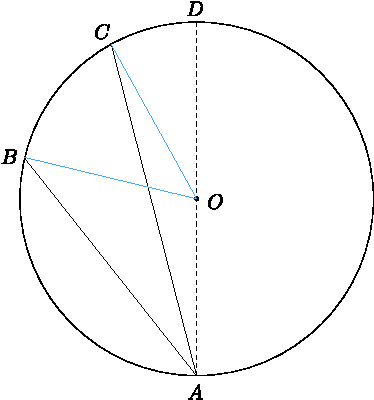
\includegraphics[scale=1]{fig/107a.pdf}
	%\caption{}
\end{figure}
In the tangential case, we simply have to define the angle $\angle TAB$, where $T$ is a point outside the circle tangent to $A$, to be the angle inscribed by $A$ and $B$, then the proof is straightforward.

\newpage

\end{document}
